\documentclass[10pt]{standalone}
% Figure 1 (architecture schematic), built as its own vector PDF so the text is real
% embedded Helvetica at 6-8pt as the journal asks. Rebuild: pdflatex fig1_architecture
\usepackage[T1]{fontenc}
\usepackage{helvet}
\renewcommand{\familydefault}{\sfdefault}
\usepackage{xcolor}
\usepackage{tikz}
\usetikzlibrary{arrows.meta,positioning,calc,fit,backgrounds}
\definecolor{ink}{HTML}{0B0B0B}
\definecolor{muted}{HTML}{898781}
\definecolor{hair}{HTML}{E1E0D9}
\definecolor{plane}{HTML}{F0EFEC}
\definecolor{memblue}{HTML}{2A78D6}
\definecolor{memorange}{HTML}{EB6834}
\begin{document}
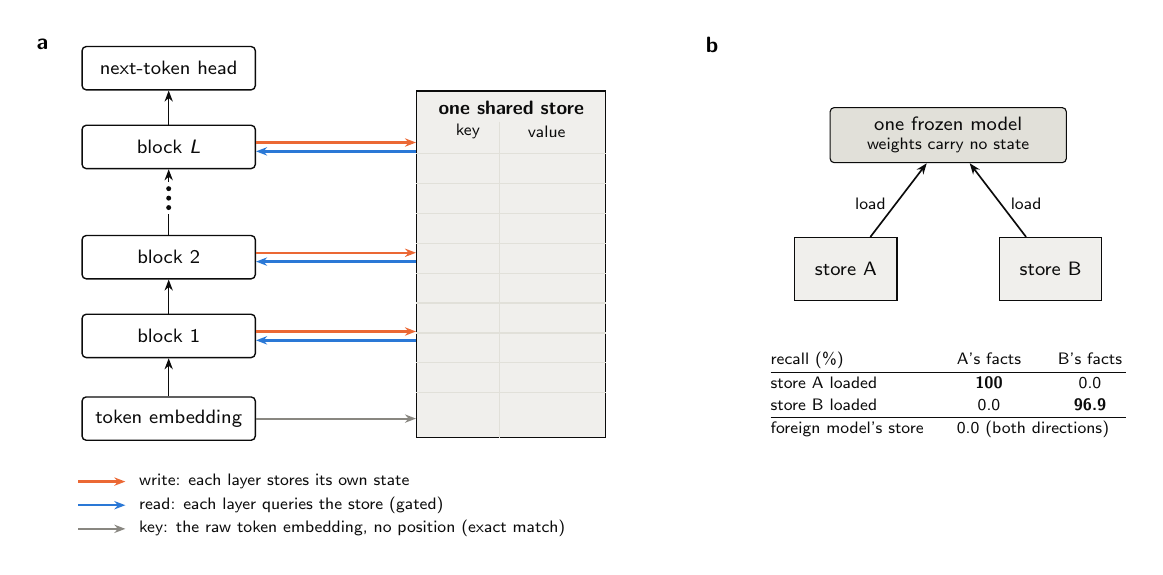
\begin{tikzpicture}[font=\sffamily\fontsize{7}{8}\selectfont, >={Stealth[length=4pt]},
  blk/.style={draw=ink, fill=white, rounded corners=1.5pt, minimum width=22mm,
              minimum height=5.5mm, line width=0.5pt, text=ink},
  note/.style={text=ink, align=left, font=\sffamily\fontsize{6}{7}\selectfont}]
  % panel a: the block
  \node[font=\sffamily\fontsize{8}{9}\selectfont\bfseries] at (-1.6,4.75) {a};
  \node[blk] (emb) at (0,0)   {token embedding};
  \node[blk] (b1)  at (0,1.05) {block 1};
  \node[blk] (b2)  at (0,2.05) {block 2};
  \node[inner sep=0pt] (dots) at (0,2.8) {\rule{0pt}{4mm}};
  \foreach \dy in {-0.12,0,0.12} \fill[ink] (0,2.8+\dy) circle (0.9pt);
  \node[blk] (bL)  at (0,3.45) {block \textit{L}};
  \node[blk] (head) at (0,4.45) {next-token head};
  \foreach \u/\v in {emb/b1, b1/b2, bL/head} \draw[->, ink, line width=0.5pt] (\u) -- (\v);
  \draw[ink, line width=0.5pt] (b2) -- (dots);
  \draw[->, ink, line width=0.5pt] (dots) -- (bL);
  % shared store
  \node[draw=ink, fill=plane, line width=0.5pt, minimum width=24mm, minimum height=44mm,
        anchor=south] (store) at (4.35,-0.25) {};
  \node[text=ink, font=\sffamily\fontsize{7}{8}\selectfont\bfseries] at ($(store.north)+(0,-0.22)$) {one shared store};
  \node[text=ink, font=\sffamily\fontsize{6}{7}\selectfont] at ($(store.north)+(-0.55,-0.52)$) {key};
  \node[text=ink, font=\sffamily\fontsize{6}{7}\selectfont] at ($(store.north)+(0.45,-0.52)$) {value};
  \draw[hair, line width=0.4pt] ($(store.north)+(-0.15,-0.4)$) -- ($(store.south)+(-0.15,0)$);
  \foreach \k in {1,...,9} \draw[hair, line width=0.4pt]
     ($(store.north west)+(0,-0.42-0.38*\k)$) -- ($(store.north east)+(0,-0.42-0.38*\k)$);
  % read / write arrows at every layer
  \foreach \b in {b1,b2,bL} {
    \draw[->, memorange, line width=0.9pt] ([yshift=1.6pt]\b.east) -- ([yshift=1.6pt]\b.east -| store.west);
    \draw[<-, memblue,   line width=0.9pt] ([yshift=-1.6pt]\b.east) -- ([yshift=-1.6pt]\b.east -| store.west);
  }
  % the address
  \draw[->, muted, line width=0.7pt] (emb.east) -- (emb.east -| store.west);
  % legend
  \draw[->, memorange, line width=0.9pt] (-1.15,-0.8) -- (-0.55,-0.8);
  \node[note, anchor=west] at (-0.5,-0.8) {write: each layer stores its own state};
  \draw[->, memblue, line width=0.9pt] (-1.15,-1.1) -- (-0.55,-1.1);
  \node[note, anchor=west] at (-0.5,-1.1) {read: each layer queries the store (gated)};
  \draw[->, muted, line width=0.7pt] (-1.15,-1.4) -- (-0.55,-1.4);
  \node[note, anchor=west] at (-0.5,-1.4) {key: the raw token embedding, no position (exact match)};

  % panel b: the store is the state
  \begin{scope}[xshift=8.3cm]
  \node[font=\sffamily\fontsize{8}{9}\selectfont\bfseries] at (-1.4,4.75) {b};
  \node[draw=ink, fill=hair, rounded corners=1.5pt, minimum width=30mm, minimum height=7mm,
        text=ink, align=center] (frozen) at (1.6,3.6) {one frozen model\\[-1pt]{\fontsize{6}{7}\selectfont weights carry no state}};
  \node[draw=ink, fill=plane, minimum width=13mm, minimum height=8mm, text=ink, align=center]
        (sa) at (0.3,1.9) {store A};
  \node[draw=ink, fill=plane, minimum width=13mm, minimum height=8mm, text=ink, align=center]
        (sb) at (2.9,1.9) {store B};
  \draw[->, ink, line width=0.6pt] (sa) -- node[note, left, pos=0.45] {load} (frozen);
  \draw[->, ink, line width=0.6pt] (sb) -- node[note, right, pos=0.45] {load} (frozen);
  \node[text=ink, align=center, font=\sffamily\fontsize{6}{7}\selectfont] at (1.6,0.3) {%
    \renewcommand{\arraystretch}{1.15}%
    \begin{tabular}{@{}lcc@{}}
      recall (\%) & A's facts & B's facts \\ \hline
      store A loaded & \textbf{100} & 0.0 \\
      store B loaded & 0.0 & \textbf{96.9} \\ \hline
      foreign model's store & \multicolumn{2}{c}{0.0 (both directions)}
    \end{tabular}};
  \end{scope}
\end{tikzpicture}
\end{document}
